\documentclass[12pt, titlepage]{article}

\usepackage{booktabs}
\usepackage{tabularx}
\usepackage{hyperref}
\usepackage{graphicx}
\hypersetup{
    colorlinks,
    citecolor=black,
    filecolor=black,
    linkcolor=red,
    urlcolor=blue
}
\usepackage[round]{natbib}

\title{SE 3XA3: Software Requirements Specification\\PasswordProtectionProgram}

\author{Team 28, Tuples1
		\\ Shabana Dhayananth dhayanas
		\\  Suhavi Sandhu sandhs11
		\\ Joseph Lu luy89
}

\date{\today}

\begin{document}

\maketitle

\pagenumbering{roman}
\tableofcontents
\listoftables
\listoffigures

\begin{table}[bp]
\caption{\bf Revision History}
\begin{tabularx}{\textwidth}{p{3cm}p{2cm}X}
\toprule {\bf Date} & {\bf Version} & {\bf Notes}\\
\midrule
Date 1 & 1.0 & Notes\\
Date 2 & 1.1 & Notes\\
\bottomrule
\end{tabularx}
\end{table}

\newpage

\pagenumbering{arabic}

This document describes the requirements for ....  The template for the Software
Requirements Specification (SRS) is a subset of the Volere
template~\citep{RobertsonAndRobertson2012}.  If you make further modifications
to the template, you should explicity state what modifications were made.

\section{Project Drivers}

\subsection{The Purpose of the Project}

The purpose of this project is to implement an encrypted password manager,  PasswordProtectionProgram (PPP) 
wherein a person can safely store and access all of the passwords they use with a single master password. 
Through working on this project the software team also hopes to learn about encryption methods and the 
development process.

\subsection{The Stakeholders}

The stakeholders of this project are:
\begin{itemize}
\item Users of online services that want a place to store their passwords safely and generate stronger passwords
\item Services for which the passwords are created as they have to deal with security threats and users that forget their passwords
\item Identity thieves since they are able to breach users’ personal information due to weak passwords and weak encryption methods
\item The development team, as they are the students attempting to solve the problem at hand
\end{itemize}

\subsubsection{The Client}

\subsubsection{The Customers}

\subsubsection{Other Stakeholders}

\subsection{Mandated Constraints}

\subsubsection{Solution Constraints}

\textbf{Description}: The product shall operate on all Operating Systems with python installed. (i.e. Windows, OSX, Linux) through a gui app.
\\
\textbf{Rationale}: The client will use all of these operating systems
\\
\textbf{Fit criterion}: The product shall be approved by testing groups of each operating system.

\subsubsection{Partner or Collaborative Applications}

The product does not have any direct partner or collaborative applications. This product is fully built on python and MariaDB and will be able to be executed in the desktop.

\subsubsection{Off-the-Shelf Software}

The off-the-shelf software required for this product to be implemented:
\begin{itemize}
\item Python
\item MariaDB
\item Tkinter (python library)
\end{itemize}
All the software that is required is open source and can be found on the internet.

\subsubsection{Budgeting Constraints}

The budget of our project is zero dollars so no further purchases are required.

\subsubsection{Schedule Constraints}

There is a deadline in December for the project to be completed.

\subsection{Naming Conventions and Terminology}
\begin{table}
\begin{center}
\begin{tabular}{ | p{3cm} | p{10cm} | }
	\hline
	Term & Definition \\
	\hline
	AES & Abbreviation for the Advanced Encryption Standard, a symmetric cipher that is implemented in the cryptography library that we will be using \\
	\hline
	Authentication & The process of verifying the identity of the user account holder  \\
	\hline
	Cipher & Another term for cryptographic algorithm \\
	\hline
	Crypographic Algorithm & A means of altering data from a readable form to a protected form (and vice-versa) \\
	\hline
	cryptography & ython library that will be used to encrypt and decrypt passwords \\
	\hline
	Dictionary Attack & A hacking technique that tries to bypass internet security by determining passwords or encryption keys using a very large number of likely possibilities \\
	\hline
	Encryption & The process of converting information or data into a code, especially to prevent unauthorized access \\
	\hline
	GUI & Graphical Use Interface \\
	\hline
	Hash & A value returned by a cryptographic hash function, a mathematical algorithm that maps data of arbitrary size to a bit string of a fixed size decreasing the likelihood of a dictionary attack \\
	\hline
	Key & A piece of information that determines the output of a cryptographic algorithm \\
	\hline
	MariaDB & A community-developed fork of the MySQL relational database management system which will be used to locally store usernames and databases \\
	\hline
	Master Password & The password that the user inputs to access the stored usernames and passwords \\
	\hline
	Module & A Python object that one can bind and reference by importing, contains definitions and statements \\
	\hline
	Padlock & The original password management software \\
	\hline
	pip3 & A package management system used to install and manage software packages for Python 3 \\
	\hline
	PPP & An abbreviation for the project, the PasswordProtectionProgram \\
	\hline
	PW & Abbreviation for password \\
	\hline
	Python 3 & The language that will be used to develop the product\\
	\hline
	random & Python module that will be used for generating passwords \\
	\hline
	Salt & A random piece of data used to enhance the one-way function that hashes a password, thereby decreasing the likelihood of dictionary attacks \\
	\hline
	Symmetric Cipher & The specific cipher that will be used for encryption, the key that it employs for going from readable form to protected form is the same \\
	\hline
	Tkinter & Python module that is going to be used to create a graphical user interface, known as Python’s standard GUI package \\
	\hline 
	Unicode & World computing standard for encoding and representing symbols and characters \\
\hline
\end{tabular}
\\
\caption{Table 1: Terminology}
\end{center}
\end{table}

\subsection{Relevant Facts and Assumptions}

Some relevant facts regarding this project are that the original program has 29850 lines of code. 
The program has a GNU General Public Licence v3.0 licence and can be run on Windows, Unix and Linux 
operating systems as well as iOS and Android mobile devices. The team will be using symmetric encryption
 from the cryptography library, which implements AES with a 128-bit key for encryption. AES is chosen by the 
U.S. government to protect classified information throughout the world to encrypt sensitive data. A relevant 
fact about passwords that has to do with the project is that passwords are easily hacked because humans 
follow similar patterns. For instance, the numbers ‘1’ and ‘2’ are common and capital letters are often used at
 the beginning of passwords. Lastly, it should be noted that the original product implemented AES and used 
PBKDF2, a key derivation function that reduces the chance of brute force attacks.
\\
\\
Some assumptions made the developers are that the cryptography library will be enough for our needs and does
 not need to be tested for its encryption since that would require executing brute force attacks. Also, it is 
assumed that there is a need for users to store their usernames and passwords safely. Lastly, it is assumed 
that Python code can run on Windows, Unix and Linux environments. 

\section{Functional Requirements}

\subsection{The Scope of the Work and the Product}

We will be re-implementing the original open source software (Padlock) as an offline, 
desktop application, suitable for Windows, Macintosh or Unix environments. This is due to time 
constraints set by the project deadline as well as further security by not having the product online. 
Also, the Python cryptography library will be used for the encryption as the development team does not 
have experience creating secure encryption methods. 

\subsubsection{The Context of the Work}

Almost all services provided to consumers, including banking, health records and social media, 
stores sensitive personal information in a password protected account. However, strong passwords are 
often easy to forget and therefore, people usually opt for weaker passwords or use the same 
one for multiple accounts. This makes them more susceptible to security threats.

\subsubsection{Work Partitioning}

\subsubsection{Individual Product Use Cases}

\begin{figure}[h]
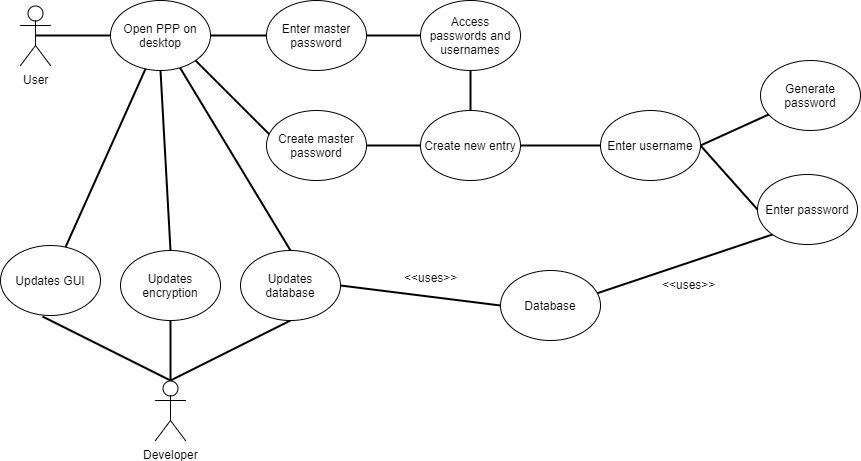
\includegraphics{Images/UseCase.png}
\caption{Figure 1: Use Case Diagram}
\end{figure}

\begin{figure}[h]
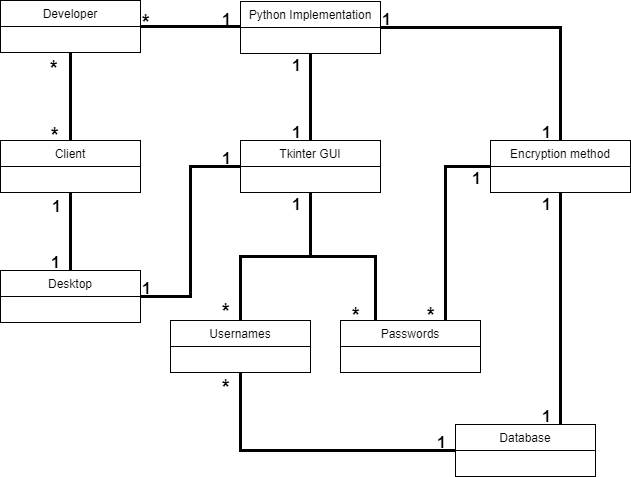
\includegraphics{Images/BusinessModel.png}
\caption{Figure 2: Business Data Model}
\end{figure}

\subsection{Functional Requirements}

\begin{center}
\begin{tabular}{ | p{1cm} | p{4cm} | p{4cm} | p{4cm} | }
	\hline
	Name & Description & Rationale & Fit Criterion\\
	\hline
	FR1 & The executaable Python code will create a user interface window & To allow user to use the application & Run application \\
	\hline
	FR2 & Upon execution, the program will have a connection to a local database & To allow the program to store usernames and encrypted passwords & Create a new entry and check if it shows up on DB \\
	\hline
	FR3 & The user must be able to create a master password & To ensure that only the user can access the data & When opening the app for the first time, create master password and use it \\
	\hline
	FR4 & The user must be able to enter a master password & To access and create passwords and usernames & Enter correct PW and incorrect PW \\
	\hline
	FR5 & The new user must be able to add a new entry & To allow the user to store a new username and password & Create new entry, close app and verify it exists in DB \\
	\hline
	FR6 & The user should be able to generate a random password & To allow for a stronger password & Generate multiple PWs and verify randomness \\
	\hline
	FR7 & The user interface must have a link to the user manual & To aid the user in using the software & Manual link should take user to manual \\
	\hline
	FR8 & After one minute of inactivity, the application should go to the home screen & To protect the users’ data & Keep app running for 1 minute \\
	\hline
	FR9 & The application should have buttons to directly copy username and password & To allow user to easily input long usernames or passwords & Copy existing password and verify that it pastes onto various text inputters \\
	\hline
	FR10 & The user should be able to change their master password & To allow the user to regularly update PW & Update PW from Settings and verify that new PW works and old one does not \\
\hline
\end{tabular}
\end{center}

\section{Non-functional Requirements}

\subsection{Look and Feel Requirements}
\begin{itemize}
	\item Requirement Number: NFR1\\
The product shall have separate sections to hold the user’s account authorizations and the creation of new user account usernames and passwords.\\
Rationale: The Main functions of the product should be displayed to follow NFR6.\\
Fit Criterion: Users are able to access the main functions immediately.\\
Priority: HIGH\\
History: Created October 6, 2017
	\item Requirement Number: NFR2\\
The product shall have separate sections to hold the user’s account authorizations and the creation of new user account usernames and passwords.\\
Rationale: The Main functions of the product should be displayed to follow NFR6.\\
Fit Criterion: Users are able to access the main functions immediately.\\
Priority: HIGH\\
History: Created October 6, 2017
	\item Requirement Number: NFR3\\
The product shall have separate sections to hold the user’s account authorizations and the creation of new user account usernames and passwords.\\
Rationale: The Main functions of the product should be displayed to follow NFR6.\\
Fit Criterion: Users are able to access the main functions immediately.\\
Priority: HIGH\\
History: Created October 6, 2017

	\item Requirement Number: NFR4\\
The product will have a minimalistic aesthetic that is easy for users to find their way around the application.\\
Rationale: User should be able to understand how the product performs.\\
Fit Criterion: There should be no more than 5 active functions that the user can see and perform at once.\\
Priority: MED\\
History: Created October 6, 2017
	\item Requirement Number: NFR5\\
The Google Material Style of the Product will create a modern and functional feel for the product.\\
Rationale: The user must want to use this app.\\
Fit Criterion: Google’s Material Design Constraints will be followed.\\
Priority: LOW\\
History: Created October 6, 2017

\end{itemize}

\subsection{Usability and Humanity Requirements}
\begin{itemize}
	\item Requirement Number: NFR6\\
The product shall be intuitive and easy to understand and use.\\
Rationale: Users must be able to use this product.\\
Fit Criterion: Majority of Users are able to store a password onto the program\\
Priority: HIGH\\
History: Created October 6, 2017

	\item Requirement Number: NFR7\\
The product shall allow for the user to be able to categorize their passwords based on the service that it is used for.\\
Rationale: Intended users have multiple accounts that may span many different parts of their lives \\
Fit Criterion: Users create sections in the application\\
Priority:LOW\\
History: Created October 6, 2017

	\item Requirement Number: NFR8\\
The user shall be able to navigate their computer.\\
Rationale: Intended users are expected to understand how to copy and paste simple text.\\
Fit Criterion: Intended users are able to use the application that meets application requirements.\\
Priority: LOW\\
History: Created October 6, 2017

	\item Requirement Number: NFR9\\
The product shall use symbols and words that are naturally understandable by the user community.\\
Rationale: The user must easily understand how to use the program as per NFR6.\\
Fit Criterion: Majority of users who use the program are able to save their username and password and generate them too.\\
Priority: LOW\\
History: Created October 6, 2017

	\item Requirement Number: NFR10\\
The product shall hide the details of its construction to the user.\\
Rationale: To follow NFR6, the product shall reveal more functions as users execute more processes.\\
Fit Criterion: The options for processes that have prerequisites are not shown on the UI until they are fulfilled\\
Priority: HIGH\\
History: Created October 6, 2017
		
\end{itemize}

\subsection{Performance Requirements}
\begin{itemize}
	\item Requirement Number: NFR11\\
The product shall respond to user input within PROCESSING-TIME when all requirements are fulfilled\\
Rationale:  Latency disrupts User Experience\\
Fit Criterion: The requirements are fulfilled under PROCESSING-TIME for majority of users.\\
Priority: HIGH\\
History: Created October 6, 2017

	\item Requirement Number: NFR12\\
The application shall be responsive and when not all requirements for a process are met,  it will display a notification or error message within ERROR-TIME.  \\
Rationale: Latency disrupts the user experience of the application and renders compromises its ease of use.  \\
Fit Criterion: The notification or error message is displayed in under ERROR-TIME for USER-TEST-PERCENTAGE of users.  \\
Priority: HIGH\\
History: Created October 6, 2017

\end{itemize}

\subsection{Operational and Environmental Requirements}
\begin{itemize}
	\item Requirement Number: NFR13\\
The Program shall run on Windows, OSX and Linux OS\\
Rationale: Users of our product will have devices on Windows, OSX and Linux.\\
Fit Criterion: The product will be approved by the testing groups of each OS and coded in a cross platform language.\\
Priority: LOW\\
History: Created October 6, 2017

\end{itemize}

\subsection{Maintainability and Support Requirements}
\begin{itemize}
	\item Requirement Number: NFR14\\
The product will be available as open source.\\
Rationale: As all of the code will be available publicly, it will be easy to update and maintain.\\
Fit Criterion: Project will be uploaded on GitLab.\\
Priority: LOW\\
History: Created October 6, 2017
\end{itemize}

\subsection{Security Requirements}
\begin{itemize}
	\item Requirement Number: NFR15\\
The product shall only store usernames and encrypted passwords.\\
Rationale: Unencrypted passwords will not be stored, all passwords will be encrypted when added to database.\\
Fit Criterion: The encrypted password is displayed to the user\\
Priority: HIGH\\
History: Created October 6, 2017

	\item Requirement Number: NFR16\\
The product shall be able to change their master password only if they are already logged into their accounts.\\
Rationale:  There will not be an email associated with the account to facilitate a reset password option on the log in page.\\
Fit Criterion: The change password option is only shown when the user is logged in already.\\
Priority: HIGH\\
History: Created October 6, 2017

	\item Requirement Number: NFR17\\
The product shall contain security measures in order to prevent the data from being accessed directly from the user’s machine by people other than the user.\\
Rationale: The user may unknowingly leave their computer unattended for a long period of time.\\
Fit Criterion: The application logs out after a certain duration of inactivity.\\
Priority: HIGH\\
History: Created October 6, 2017

	\item Requirement Number: NFR18\\
The product shall not distribute the user’s personal information to third parties.\\
Rationale: The purpose of the software is to secure the client’s personal information.\\
Fit Criterion: The personal information will not be distributed.\\
Priority: HIGH\\
History: Created October 6, 2017
	
\end{itemize}

\subsection{Cultural Requirements}
There are none applicable to this project

\subsection{Legal Requirements}

There are none applicable to this, as all referenced software is open source on github and there are no plans of liscencing the project.

\subsection{Health and Safety Requirements}
\begin{itemize}
	\item Requirement Number: NFR18\\
This application shall not contain any imagery or animation that can be harming to any human's health\\
Rationale: User satisfaction will be greatly decreased if the product may pose a threat to their health in any way.\\
Fit Criterion: Application does not contain potential visual health risks.\\
Priority: HIGH\\
History: Created October 6, 2017
\end{itemize}

\section{Project Issues}

\subsection{Open Issues}

Actions to be taken in the cases in which the user has lost access to their passwords or has lost all of their information due to hardware problems have not yet been explored. Also, the product will be implemented on a Windows operating system as that is the operating system used by all team members. It is intended that the software will work on Linux and Unix operating systems as well so but testing on those environments has not been discussed.

\subsection{Off-the-Shelf Solutions}
\begin{table}
\begin{center}
\begin{tabular}{ | p{3cm} | p{10cm} | }
	\hline
	Existing Product & Key Features \\
	\hline
	Padlock (template software) & Template open source software upon which the product will be based, Chrome and mobile application available \\
	\hline
	Encryptr & Cloud-based password manager \\
	\hline
	KeePass & Password database is locked with a master key or key file, encrypted with AES and Twofish \\
	\hline
	RatticDB & Intended for tracking shared  passwords among a group of employees, no application level encryption \\
\hline
\end{tabular}
\\
\caption{Table 3: Off-the-Shelf Solutions}
\end{center}
\end{table}


\subsection{New Problems}

If users solely on this product to store all of their passwords, there is potential for them to lose all of their saved data due to a hashing issue, hardware issue or in the theft or loss of their computer. The product requires that the user to enter their current master password in order to change it which could cause issues in the case that they forget it.

\subsection{Tasks}

Deliverables as outlined by SFWRENG 3XA3 courseware:

\begin{table}
\begin{center}
\begin{tabular}{ | p{5cm} | p{9cm} | }
	\hline
	Deilverable & Deadline \\
	\hline
	Requirements Document (Revision 0) & October 6, 2017 \\
	\hline
	Proof of Concept Demonstration & October 16, 2017 (week) \\
	\hline
	Test Plan (Revision 0) & October 27, 2017 \\
	\hline
	Design and Document (Revision 0) & November 10, 2017 \\
	\hline
	Demonstration (Revision 0) & November 13, 2017 (week) \\
	\hline
	Final Demonstration (Revision 1) & November 27, 2017 (week) \\
	\hline
	Final Documentation & December 6, 2017 \\
\hline
\end{tabular}
\\
\caption{Table 4: Deliverables}
\end{center}
\end{table}

Implementation Breakdown:

\begin{table}
\begin{center}
\begin{tabular}{ | p{5cm} | p{10cm} | }
	\hline
	Task & Intended Completion Date \\
	\hline
	System Design & October 12, 2017 \\
	\hline
	User Interface & October 18, 2017 \\
	\hline
	Prototype 1 & October 18, 2017 \\
	\hline
	Test 1 & October 26, 2017 \\
	\hline
	Test 1 Fixes & October 30, 2017 \\
	\hline
	Encryption & November 7, 2017 \\
	\hline
	Prototype 2 & November 13, 2017 \\
	\hline
	Test Plan Revision (Test 2) & November 16, 2017 \\
	\hline
	Test 2 Fixes & November 23, 2017 \\
	\hline
	User Guide & December 1, 2017 \\
\hline
\end{tabular}
\\
\caption{Table 5: Implementation Breakdown}
\end{center}
\end{table}

The team will be implementing and testing non-functional requirements based on their priority.

\subsection{Migration to the New Product}

The final product will be run and installed via an executable Python file. As MariaDB will be used to store the usernames and passwords, the database will have to be converted before the product is released. It also needs to be tested on all intended operating systems.

\subsection{Risks}

Security is the main concern for this project as the team is not explicitly testing the strength of the encryption method under the assumption that the cryptography library is reliable. The probability of this becoming a problem is unlikely as the product will be offline and will not be a target of many attacks. If the problem does occur, the team will look into a more complex encryption method. 

\subsection{Costs}

Not applicable in the case that all required dependencies are open-source or free.

\subsection{User Documentation and Training}

There will be a concise and useful manual that provides instructions on how to use the product. To make the product easier to use, the team will be testing for the GUI’s user-friendliness and receiving feedback from others. 

\subsection{Waiting Room}

Ideally, there would be a backup data option for the user to use as a precaution in the case of hardware 
failure and loss of data.
\\
To improve the user interface, it would be nice to provide support for multiple languages (other than only English).
\\
Passwords can be organized by service in the database, so based on that there can be different levels of security provided. For example, bank passwords and library account passwords don’t need the same level of security.

\subsection{Ideas for Solutions}

Instead of storing passwords, another solution is 2 factor authentication (2FA). This eliminates the need to download a password management software and instead the user can do a phone verification after typing their password or a fingerprint scanner for mobile devices.

\begin{figure}[h]
\includegraphics{Images/2fa.png}
\caption{Figure 3: 2 Factor Authentication}
\end{figure}

\bibliographystyle{plainnat}

\bibliography{SRS}

\newpage

\section{Appendix}

This section has been added to the Volere template.  This is where you can place
additional information.

\subsection{Symbolic Parameters}

The definition of the requirements will likely call for SYMBOLIC\_CONSTANTS.
Their values are defined in this section for easy maintenance.


\end{document}
